\chapter{Introduction}
\label{chapter:introduction}

% possiveis estruturas
% Motivação, Objetivos, Challenges, Estrutura
% Background, Motivation and objectives, Structure

\section{Background}

The Third Industrial Revolution was characterized by a focus on automating repetitive and heavy tasks on the assembly lines. Still, this created a problem: whenever the manufacturers needed the robots to work in a different assembly process, they needed to be reprogrammed by an expert.

The Fourth Industrial Revolution, also known as Industry 4.0, refers to the current trend of the manufacturing sector to become more intelligent and achieve greater automation. This trend takes advantage of the recent developments in artificial intelligence, the Internet of Things, and autonomous robots to pave the way for more efficient and flexible production processes. With Industry 4.0, robots are expected to be more adaptable and perform more actions without constant explicit programming.

The concept of \acf{hrc} emerges as part of Industry 4.0 and involves the research of mechanisms that allow humans and robots to work together to achieve a shared goal. Some of the most relevant mechanisms in recent research include collision avoidance and human-aware planning of robot motions. However, to achieve true collaboration it is not enough to react to the partner's movements and intentions, the robot must anticipate them.

\acf{ai} has significantly evolved in the last years. With the increase of computational power, Machine Learning, a subset of \acs{ai}, has become an increasingly promising method to deal with complex data like images and text heavily contributing to areas such as visual perception and speech recognition. Machine Learning's ability to learn from data with minimal human intervention and understand new data it has never seen before make it a prime candidate to solve many problem in robotics and \acs{hrc} in particular.

This work attempts to use state-of-the-art machine learning techniques to tackle the problem of action anticipation.

\if{0}
To better visualize the real-world application, suppose, for example, that a human worker needs a specific material, such as a wooden plank. In this case, the robot can anticipate it and either provide it as it did in Fig.~\ref{example} or move out of the way to avoid a collision. Furthermore, anticipating human actions helps improve the overall speed and manufacturing efficiency of the collaborative assembly while also helping to reduce the risk of accidents or injuries, increasing safety.

\begin{figure}[htbp]
\centerline{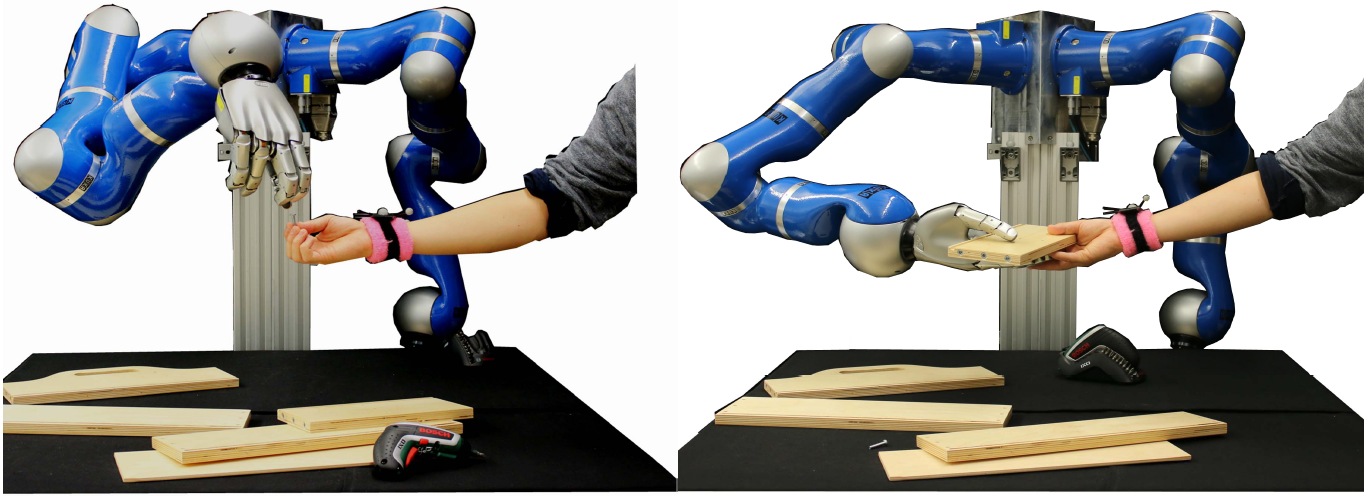
\includegraphics[width=3.5in]{figs/example.PNG}}
\caption{Situation where a robot anticipates that the worker will need a wooden plank and hands it over to him \cite{Maeda2016}}
\label{example}
\end{figure}
\fi

%\section{Motivation}

\section{Problem Definition}

This dissertation aims at the development of an action anticipation system to enhance human-robot collaboration in industrial settings under the AUGMANITY mobilizing project.

Action anticipation is a technique that can be used in collaborative assembly so that robots predict the next actions of their human collaborators and respond accordingly. In the robot's perspective this results in a better coordination of its own movements and actions to efficiently and safely work with the human.

Subsequently, the main objectives of this work can be summarized as follows:

\begin{itemize}
\item Development of a machine learning model to infer the next action in a human-robot collaborative scenario. This includes data gathering, model training and optimization.
\item Development of an anticipatory robot controller. It must consider the inferred action and the partners movements to make the best action during the execution of a sequential assembly task.
\item Metrics and performance evaluation. To provide performance metrics used to evaluate the action anticipation models and the add-value of the anticipatory controller (e.g., in terms of cycle time).
\end{itemize}

\section{Structure}

This document is composed of six chapters as follows:

\begin{itemize}
\item Chapter \ref{chapter:introduction} - Introduction.
\item Chapter \ref{chapter:state_of_the_art} - State of the Art containing background material about anticipation, machine learning and collaborative robotics and a review of previous work on Action Anticipation in HRC including data sources, algorithms and safety measures.
\item Chapter \ref{chapter:tools_review} - Tools Review containing a review of tools that can be useful in the implementation.
\item Chapter \ref{chapter:work_progress} - Work progress made in the first semester.
\item Chapter \ref{chapter:planning} - Planning of the second semester work.
\item Chapter \ref{chapter:conclusion} - Conclusion.
\end{itemize}
